\documentclass[presentation]{subfiles}
\onlyinsubfile{
  \bibliography{references}
  \usepackage{tikz}
  \usetikzlibrary{positioning}
\renewcommand{\onlyinsubfile}[1]{}

}

\begin{document}


\begin{frame}{
  on--demand work's limits
}
  
  % While algorithms will increase the complexity ceiling beyond what was possible previously with piecework, there's essentially a fundamental limit to how complex such work can become.

  % Technology’s ability to support human cognition will enable stronger assumptions about workers’ abilities, increasing the complexity of on–demand work outcomes.

  % \begin{center}
  % \end{center}

  \visible<1->{
  \begin{columns}
  \begin{column}{0.5\textwidth}
  
    \begin{center}
      We'll be able to make stronger assumptions of what people know
    \end{center}
  
  % \vspace{1em}

  \includegraphics[width=\textwidth]{../../common_figures/photo/knowledge-student.png}

  \end{column}
  \begin{column}{0.5\textwidth}
  % \begin{figure}
  % \only<2>{
  % \includegraphics[width=\textwidth]{../../common_figures/complexity/brain_scansA.png}
  % }


  \visible<2->{
  
  \visible<3->{\begin{center}
    \dots but we probably won't be able to get much further than piecework did.
    \end{center}}

  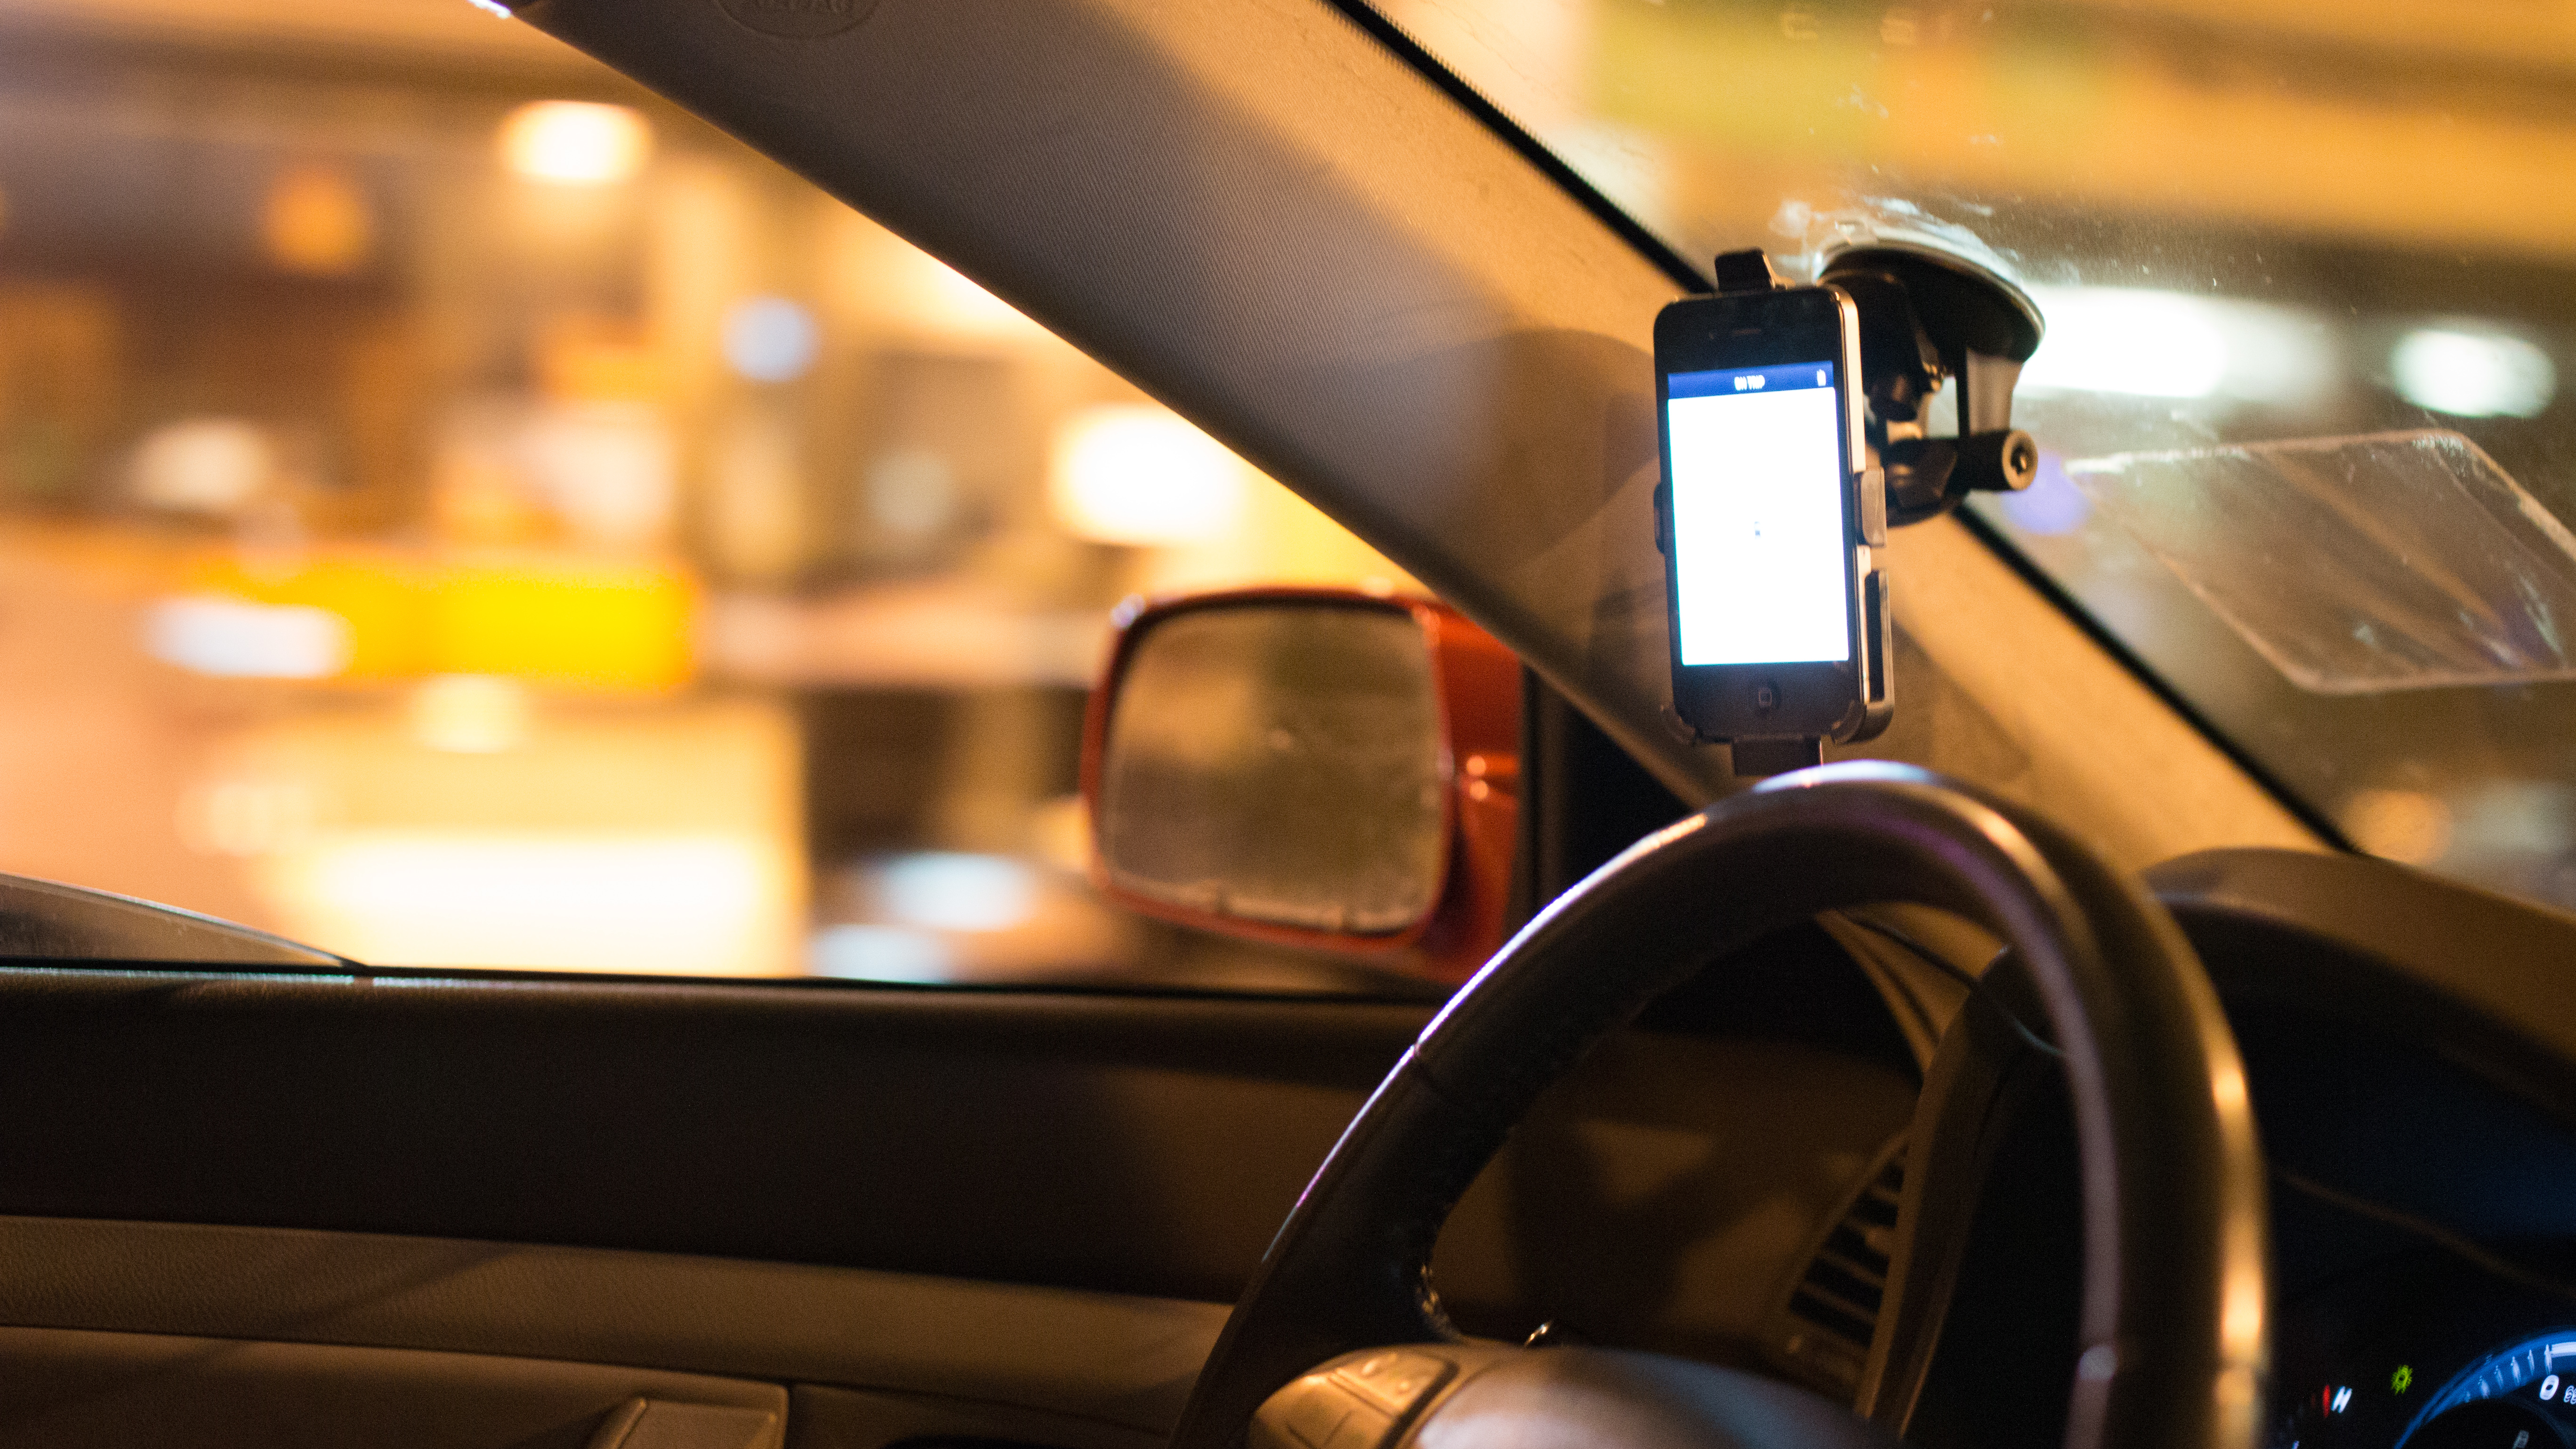
\includegraphics[width=\textwidth]{../../common_figures/photo/gps-map.png}}
  % \end{figure}
  \end{column}
  \end{columns}
  }




\end{frame}

% \section{Piecework\\
% {\hfill\footnotesize\citeauthor{pieceworkCrowdworkGigwork} @ \citefield{pieceworkCrowdworkGigwork}{series}}}
% \subfile{piecework/introduction}
% \subfile{piecework/piecework-simple}
% \subfile{piecework/piecework-complex}


\end{document}